%%%%%%%%%%%%%%%%%%%%%%%%
%
% $Autor: Sadegh Naderi $
% $Datum: 2023-11-24  $
% $Directory: ML23-01-Keyword-Spotting-with-an-Arduino-Nano-33-BLE-Sense/report/Contents/en/DataTransformandMining.tex $
% $Version: 3 $
% $Review by: Achal Shakywar, Sadegh Naderi $
% $Review date: 2024-02-11 $
%
%%%%%%%%%%%%%%%%%%%%%%%%

\chapter{Data Transformation and Data Mining in \ac{kdd}}


\section{Data Transformation}
\label{section:DataTransformation}

As was discussed in the Section \ref{subsection:InputDataSpeech} the raw audio files are converted to spectrograms. Here, more technical aspects of the conversion are discussed here.

\subsection{How Does Feature Generation Function?}

The method employed mirrors the one utilized throughout Google's production processes, underscoring its substantial practical validation. The theoretical view was discussed in the section \ref{subsection:convertAudio}. Here, we provide a general overview of its functioning. 
The procedure initiates by creating a Fourier transform (also referred to as fast Fourier transform or FFT) for a specific time segment—30 ms of audio data in our case. This FFT is generated on data subjected to a Hann window, a bell-shaped function diminishing the impact of samples at the window's ends. The Fourier transform yields complex numbers with real and imaginary components for every frequency. However, our focus is on overall energy, so we sum the squares of the components and apply a square root to obtain magnitudes for each frequency bucket \cite{Warden:2019}.

With N samples, a Fourier transform provides information on N/2 frequencies. For a 30-ms duration at a 16,000 samples-per-second rate, 480 samples are required. As our FFT algorithm necessitates a power-of-two input, we pad it with zeros to 512 samples, resulting in 256 frequency buckets. To reduce this, we average adjacent frequencies into 40 downsampled buckets. This downsampling utilizes the mel frequency scale, which is perception-based, assigning more weight to lower frequencies. This process merges higher frequencies into broader buckets, as depicted in Figure \ref{fig:featureGeneration}. The output of this process was shown in the Figure \ref{fig:SpectralYesNoCombined}.

\begin{figure}[h!]
	\centering
	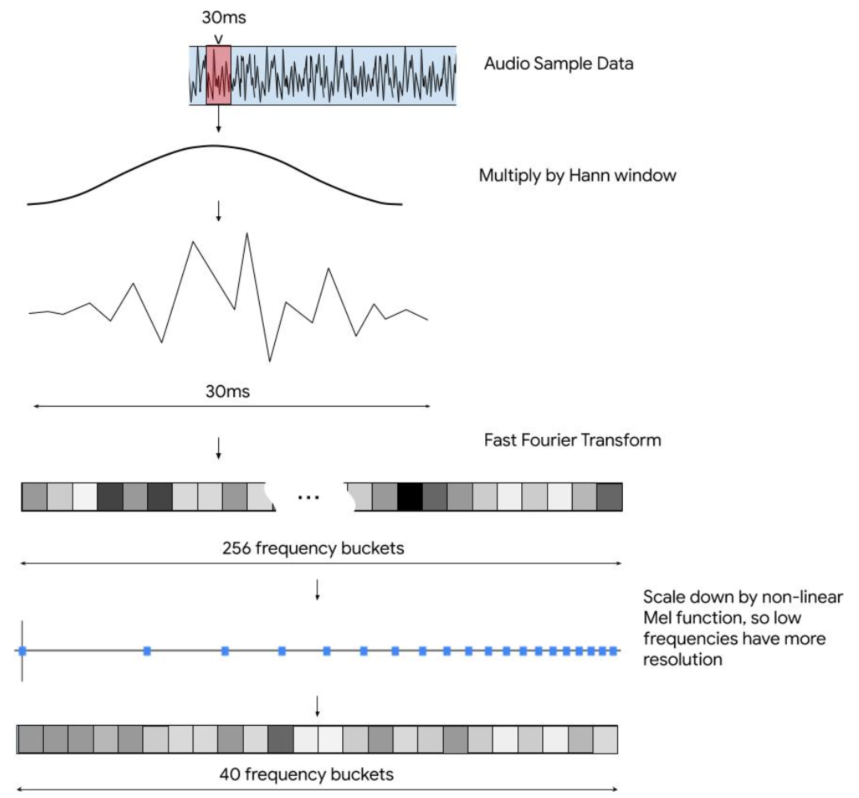
\includegraphics[width=0.8\textwidth]{Images/KDDProcess/featureGeneration}
	\caption{Feature-generation process diagram \cite{Warden:2019}.} \label{fig:featureGeneration}
\end{figure}

A distinctive aspect of this feature generator is its inclusion of a noise reduction step. This involves maintaining a running average for each frequency bucket and subtracting this average from the current value. The goal is to eliminate background noise, which tends to be constant, leaving the speech signals intact. The feature generator retains state to track running averages, necessitating state reset for consistent spectrogram reproduction.

Surprisingly, the noise reduction involves different coefficients for odd and even frequency buckets, creating comb-tooth patterns in the final feature images. Initially perceived as a bug, it was intentionally added to enhance performance. Empirical testing confirmed its impact on accuracy.

Per-channel amplitude normalization (PCAN) auto-gain is applied to boost the signal based on running average noise. Finally, a log scale is employed for all bucket values, preventing loud frequencies from overpowering quieter portions—a normalization aiding the subsequent model's interaction with features.

This entire process is iterated 49 times, employing a 30-ms window moved forward by 20 ms between iterations, covering one second of audio input data. The result is a 2D array of values, 40 elements wide (one for each frequency bucket) and 49 rows high (one for each time slice).


\section{Data Mining and the Model}

The neural network model we utilize is delineated as a concise graph of operations, with Figure \ref{fig:SpeechRecognitionModelGraph} providing a visual representation of the model structure. This model encompasses a convolutional layer, succeeded by a fully connected layer, and concludes with a softmax layer. While the convolutional layer is denoted as "DepthwiseConv2D" in the figure, this nomenclature is a quirk of the TensorFlow Lite converter. It is revealed that a convolutional layer with a single-channel input image can be expressed as a depthwise convolution. Additionally, a layer labeled "Reshape\_1" serves as an input placeholder rather than an actual operation \cite{Warden:2019}.


\begin{figure}[h!]
	\centering
	%%%%%%%%%%%%%%%%%%%%%%%%
%
% $Author: Sadegh Naderi $
% $Datum: 13.12.2023  $
% $Pfad: MLProject\ML23-01-Keyword-Spotting-with-an-Arduino-Nano-33-BLE-Sense\report\Images\KDDProcessSpeechRecognitionModelGraph.tex $
% $Version: 1.0 $
%
% !TeX encoding = utf8
%
%%%%%%%%%%%%%%%%%%%%%%%%

\usetikzlibrary{arrows.meta}

\begin{tikzpicture}[
	node distance=2cm,
	block/.style={rectangle, draw, text width=5cm, text centered, minimum height=1cm},
	arrow/.style={->, >=Stealth}
	]
	% Nodes
	\node [block] (reshape) {reshape\_1};
	\node [block, below=of reshape] (conv) {\textbf{DepthwiseConv2D} \\ weights $<1 \times 10 \times 8 \times 8>$ \\ bias $<8>$};
	\node [block, below=of conv] (fc) {\textbf{FullyConnected} \\ weights $<4 \times 4000>$ \\ bias $<8>$};
	\node [block, below=of fc] (softmax) {Softmax};
	\node [block, below=of softmax] (labels) {labels\_softmax};
	
	% Arrows
	\draw [arrow] (reshape) -- (conv) node[midway, right] {$1 \times 49 \times 40 \times 1$};
	\draw [arrow] (conv) -- (fc) node[midway, right] {$1 \times 25 \times 20 \times 8$};
	\draw [arrow] (fc) -- (softmax) node[midway, right] {$1 \times 4$};
	\draw [arrow] (softmax) -- (labels) node[midway, right] {$1 \times 4$};
\end{tikzpicture}

	\caption{Visual representation of the speech recognition model's graph} \label{fig:SpeechRecognitionModelGraph}
\end{figure}


Convolutional layers are employed to identify 2D patterns in input images. Each filter, a rectangular array of values, functions as a sliding window across the input, generating an output image that reflects the similarity between the input and filter at each point. The convolution operation can be conceptualized as moving rectangular filters across the image, with each filter's result indicating its similarity to the corresponding image patch. In this instance, each filter is 8 pixels wide and 10 pixels high, with a total of 8 filters. The filters are shown in the Figure \ref{fig:filterImages}.

\begin{figure}[h!]
	\centering
	
	\begin{subfigure}{0.22\textwidth}
		
\includegraphics[width=\linewidth]{Images/KDDProcess/firstFilter}
		\caption{}    % \caption{} is kept to keep (a), (b), (c) etc. below each subfigure.
		\label{subfig:firstFilter}
	\end{subfigure}
	\hfill
	\begin{subfigure}{0.22\textwidth}
		
\includegraphics[width=\linewidth]{Images/KDDProcess/secondFilter}
		\caption{}    % \caption{} is kept to keep (a), (b), (c) etc. below each subfigure.
		\label{subfig:secondFilter}
	\end{subfigure}
	\hfill
	\begin{subfigure}{0.22\textwidth}
		
\includegraphics[width=\linewidth]{Images/KDDProcess/thirdFilter}
		\caption{}    % \caption{} is kept to keep (a), (b), (c) etc. below each subfigure.
		\label{subfig:thirdFilter}
	\end{subfigure}
	\hfill
	\begin{subfigure}{0.22\textwidth}
		
\includegraphics[width=\linewidth]{Images/KDDProcess/fourthFilter}
		\caption{}    % \caption{} is kept to keep (a), (b), (c) etc. below each subfigure.
		\label{subfig:fourthFilter}
	\end{subfigure}
	
	\medskip
	
	\begin{subfigure}{0.22\textwidth}
		
\includegraphics[width=\linewidth]{Images/KDDProcess/fifthFilter}
		\caption{}    % \caption{} is kept to keep (a), (b), (c) etc. below each subfigure.
		\label{subfig:fifthFilter}
	\end{subfigure}
	\hfill
	\begin{subfigure}{0.22\textwidth}
		
\includegraphics[width=\linewidth]{Images/KDDProcess/sixthFilter}
		\caption{}    % \caption{} is kept to keep (a), (b), (c) etc. below each subfigure.
		\label{subfig:sixthFilter}
	\end{subfigure}
	\hfill
	\begin{subfigure}{0.22\textwidth}
		
\includegraphics[width=\linewidth]{Images/KDDProcess/seventhFilter}
		\caption{}    % \caption{} is kept to keep (a), (b), (c) etc. below each subfigure.
		\label{subfig:seventhFilter}
	\end{subfigure}
	\hfill
	\begin{subfigure}{0.22\textwidth}
		
\includegraphics[width=\linewidth]{Images/KDDProcess/eighthFilter}
		\caption{}    % \caption{} is kept to keep (a), (b), (c) etc. below each subfigure.
		\label{subfig:eighthFilter}
	\end{subfigure}
	
	\caption{Filter images \cite{Li:2021} (\subref{subfig:Sigmoid}) First filter image  (\subref{subfig:Tanh}) Second filter image (\subref{subfig:ReLU}) Third filter image (\subref{subfig:LeakyReLU}) Fourth filter image (\subref{subfig:PReLU}) Fifth filter image (\subref{subfig:ELU}) Sixth filter image  (\subref{subfig:Swish}) Seventh filter image (\subref{subfig:Mish}) Eighth filter image}
	\label{fig:filterImages}
\end{figure}

These filters can be viewed as small patches of the input image, aiming to match them with similar sections of the input. High values are written into the corresponding part of the output image where the input resembles the patch. Each filter represents a pattern learned by the model during training to distinguish between different classes. With eight filters, eight distinct output images are produced, each corresponding to the match values of the respective filter as it traverses the input. These outputs are consolidated into a single output image with eight channels.

The subsequent operation involves a fully connected layer, which employs a different pattern matching approach. Instead of sliding a small window, there is a weight for every value in the input tensor, providing an indication of how closely the input aligns with the weights. This is a global pattern matching process, with each class having its own weights, generating four output values for classes like "silence," "unknown," "yes," and "no." The input tensor contains 4,000 values (25 * 20 * 8), representing each class with 4,000 weights.

The final layer is a softmax (explained in the section \ref{subsection:outputCNN}), enhancing the distinction between the highest output and its competitors. While the term "probability" is informally used, it requires additional calibration for reliable application. The distribution of training data influences the raw scores, and without proper calibration, it may not accurately reflect the likelihood of certain words.

In addition to these primary layers, biases are incorporated into the results of the fully connected and convolutional layers to fine-tune their outputs. A rectified linear unit (ReLU) activation function follows each layer, ensuring no output is below zero and expediting the convergence of the training process.


\section{Conclusion}

Identifying spoken words efficiently with limited memory space poses a challenging real-world task, demanding engagement with a more extensive set of components compared to simpler instances. The landscape of production machine learning applications necessitates addressing complexities such as feature generation, selecting model architectures, data augmentation, identifying optimal training data, and devising strategies to translate model outcomes into actionable insights. Depending on the product's specific needs, various trade-offs come into play \cite{Warden:2019}. The next step is the transition from the development phase to deployment.


